\RequirePackage{plautopatch}
\RequirePackage[l2tabu, orthodox]{nag}

\documentclass[dvipdfmx]{jlreq}
\usepackage{graphicx}
\usepackage{bxtexlogo}
\usepackage{float}
\usepackage{url}

\title{オブジェクト指向プログラミングレポート課題}

\author{5422007 千本木悠
 5422009 本江拓海 5422020 池田悠星}
\date{\today}

\begin{document}
\maketitle

\section{システムの概要}
プレイヤーから発射される銃弾はキーボードのZを押すことで発射される.プレイヤーはマウスで動かすことが可能である.敵に銃弾が当たると敵のHPバーが減少する.HPバーが0になると敵は消滅する.敵の球がプレイヤーに当たるとプレイヤーの残機が減少する.敵のzakoは動くようにした.

\section{クラス設計の指針}
GameObjectクラスですべてのオブジェクトを管理することにし,Character,HPBar,Bulletの3つに分けた.CharacterクラスではEnemy,Playerの2つに分けEnemyクラスではZako,Bossといったクラス設計を行った.

\section{クラス設計の詳細}
GameObjectクラスはゲーム内のオブジェクトを表す抽象クラスで,位置,サイズ,速度,色などの属性を持つ。このクラスはオブジェクトの移動や状態の管理を行うメソッドを提供する.

BulletクラスはGameObjectを継承し,ゲーム内でキャラクターが発射する弾丸を表す。弾丸がどのキャラクターに所有され,どのキャラクターにダメージを与えるかを示す属性を持ち,弾丸の攻撃力も設定できる。taskメソッドで移動を行い,一定時間後に弾丸をゲームから取り除く.

HPBarクラスはGameObjectを継承し,ゲーム内でキャラクターやオブジェクトの体力を視覚的に表示するためのUI要素を表す.現在のHPと最大HPを保持し,drawメソッドでHPの割合に応じた長さの矩形を描画する.

TextLabelクラスは,GameObjectを継承し,ゲーム内のテキスト表示を扱うUI要素を表す.文字列,フォントスタイル,文字列の左オフセットを管理し,draw メソッドで指定された位置にテキストを描画する.

Enemyクラスは,Characterクラスを継承し,ゲーム内でプレイヤーと対峙する敵キャラクターを表す.HPを示すhealth属性を持ち,collidedメソッドで弾丸との衝突を処理,弾丸の攻撃力に応じて敵の体力を減少させる。弾丸が敵に命中した場合,その弾丸をゲームから削除する。

Playerクラスは,Characterクラスを継承し,ゲーム内のプレイヤーキャラクターを表す.プレイヤーのライフを示すremaining属性を持ち,shootメソッドで敵に向けて弾丸を発射する.collidedメソッドで弾丸や敵キャラクターとの衝突を処理し,ライフを減少させる.また、taskメソッドで一定間隔ごとに弾丸を発射し,ライフがゼロになったときの処理を管理する.

ZakoクラスはEnemyクラスを継承し、ゲーム内の雑魚敵キャラクターを表す。HPBarオブジェクトを持ち,敵の現在の体力を視覚化する。shootメソッドでプレイヤーに向けて弾を発射し,taskメソッドで一定間隔での射撃と,時間経過による移動を行う.drawメソッドは敵の姿とHPバーを描画し,HPがゼロになった際に自身とHPバーをゲームから削除する.

BossクラスはEnemyクラスを継承し,ゲーム内のボスキャラクターを表す.このクラスはボスが特定のパターンで弾丸を発射するメカニズムを提供する.HPBarオブジェクトを使ってボスの体力を表示し,shootメソッドでは同心円状に弾丸を発射する.taskメソッドでは,特定の間隔で射撃を行い,HPがゼロになるとボスとHPバーをゲームから削除する.drawメソッドはボスの姿を描画する.

\begin{figure}
  \centering
  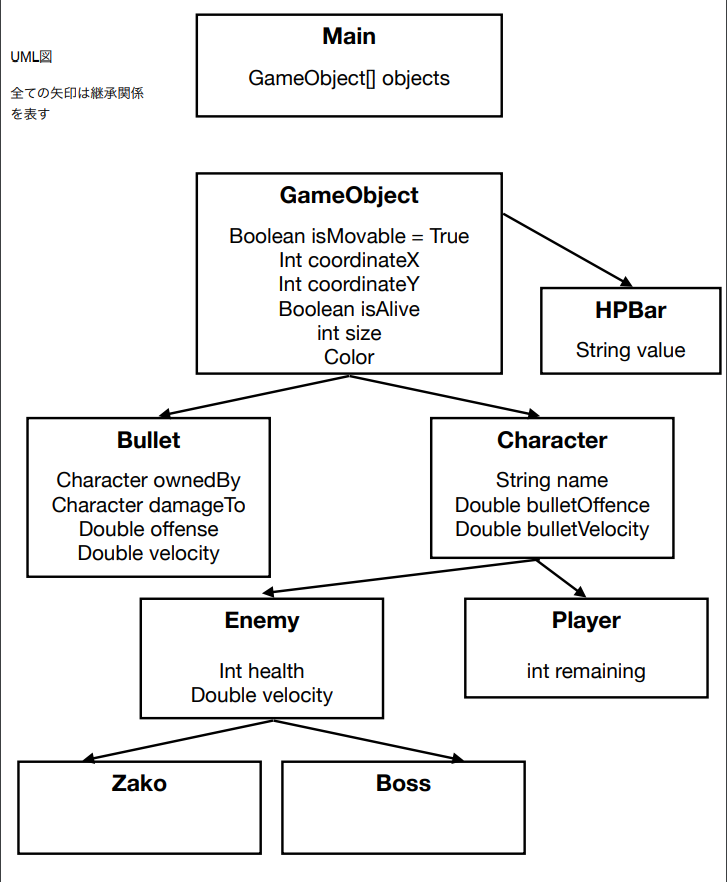
\includegraphics[width=70mm]{figures/class.png}
  \caption{クラス設計図}
  \label{fig:model}
\end{figure}

\section{実行結果}
図2の画面からスタートする.図3のように球が発射されダメージを与えた分HPバーが減少する.図4はすべての敵を倒した状態である.
\begin{figure}[H]
\centering
\begin{minipage}[b]{0.32\columnwidth}
    \centering
    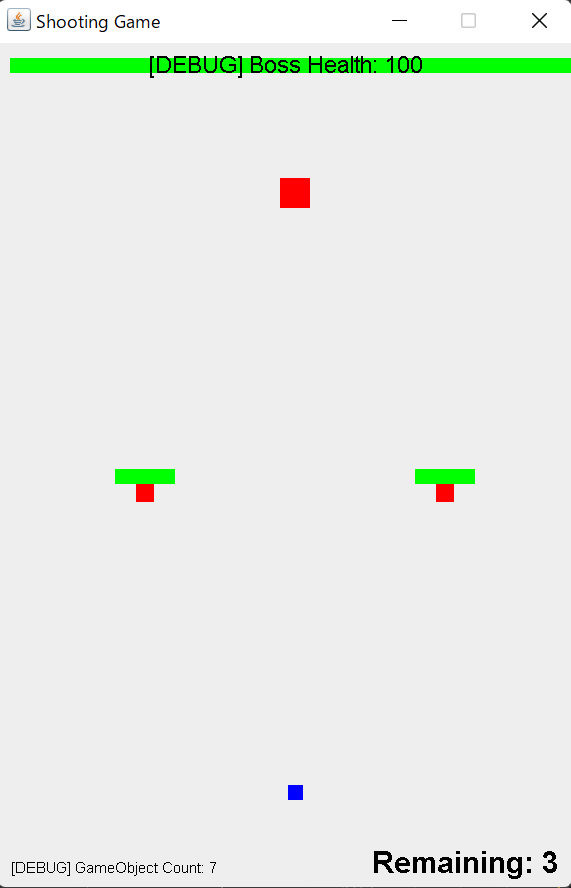
\includegraphics[width=0.7\columnwidth]{figures/result1.png}
    \caption{実行画面1}
    \label{fig:a}
\end{minipage}
\begin{minipage}[b]{0.32\columnwidth}
    \centering
    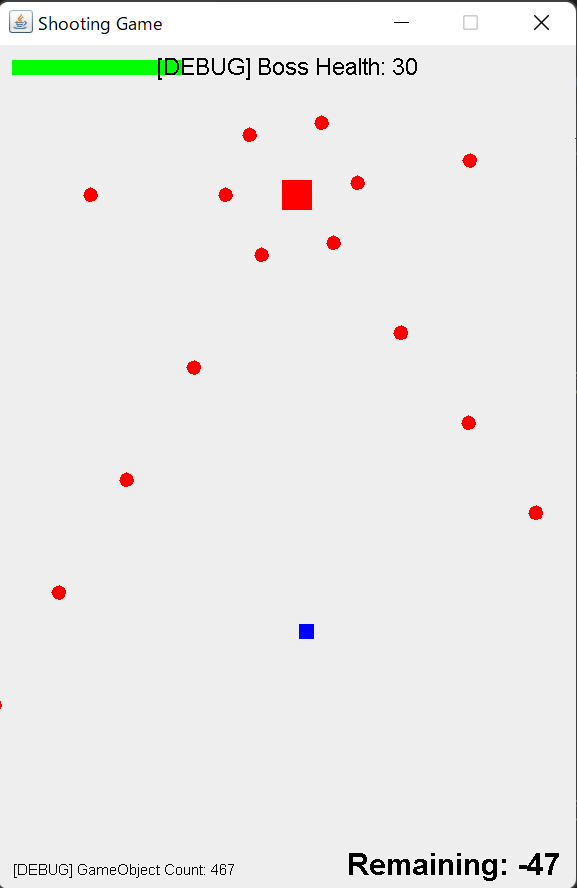
\includegraphics[width=0.7\columnwidth]{figures/result3.png}
    \caption{実行画面2}
    \label{fig:b}
\end{minipage}
\begin{minipage}[b]{0.32\columnwidth}
    \centering
    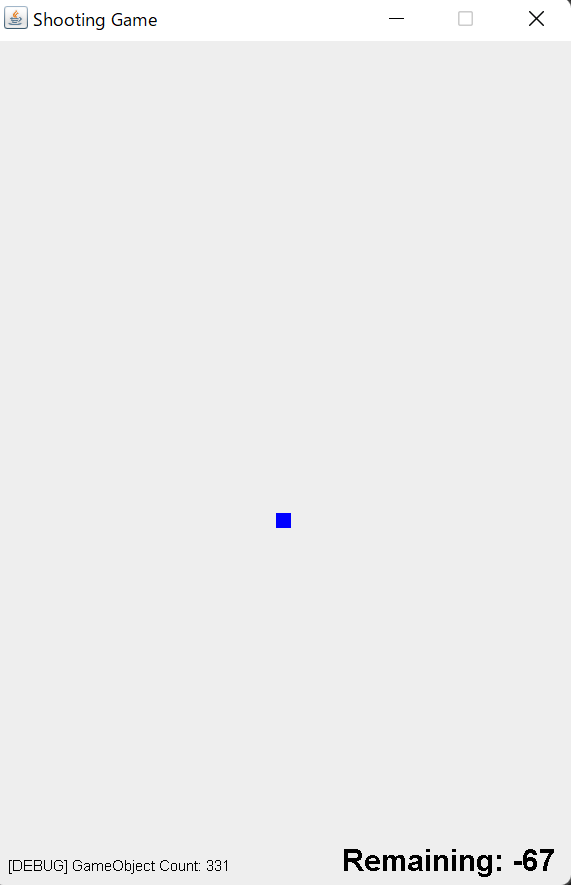
\includegraphics[width=0.7\columnwidth]{figures/result4.png}
    \caption{実行画面3}
    \label{fig:c}
\end{minipage}
\end{figure}

\section{クラス設計に対する考察}
今回のクラス設計では保守性,可読性ともに高まったといえる.GameObjectクラスから,Characterクラス,HPBarクラス,Bulletクラスに分けたことでそれぞれの管理がしやすくなりコードの可読性も高まった.また,新たに中ボスをつくる際もEnemyクラスがあることでコードの追加が容易である.

\section{ソースコード}
コードをGitHubに掲載した.URLを以下に示す.

\url{https://github.com/Piertotum-Locomotor/kthr_shooting}
\section{担当箇所}
\begin{table}[hbtp]
  \caption{執筆者らの寄与}
  \label{contribution}
  \centering
  \begin{tabular}{|c|c|}
    \hline
    内容 & 名前 \\
    \hline\hline
    レポート本文作成 & 千本木,本江 \\
    \hline
    クラス設計 &  千本木,池田\\
    \hline
    AIによる雛形作成 & 池田 \\
    \hline
    プログラミング & 千本木,本江,池田 \\
    \hline
    \LaTeX 化 & 本江\\
    \hline
  \end{tabular}
\end{table}


\end{document}